\clearemptydoublepage
\chapter{Modules}
\label{cha:modules}


The \emph{OpenCMISS} library dynamically links to a number of 
other libraries, these libraries are either externally provided 
libraries (for example: the \emph{PETSc} solver library or the 
\emph{ParMETIS} library) or internal provided libraries (the 
\emph{CellML} and \emph{FieldML} projects). 

The \emph{OpenCMISS} library itself is subdivided into a collection modules,
this section provides an introduction to each of these modules.


\section{Definitions}
\label{sec:definitions}

\emph{Class}, \emph{type} and \emph{sub-type} - In \emph{OpenCMISS}, 
\emph{class} is the broadest grouping, it is a means of identifying 
equations of a physics type (for example: \emph{Fluid Mechanics}), 
\emph{type} refers to a particular equation in that \emph{class} 
(for example: \emph{Navier Stokes}), and \emph{sub-type} refers to 
an implementation of that equation (for example: 
\emph{static Navier Stokes}). \\

\noindent Variable, parameter and routine naming - \emph{OpenCMISS} uses 
descriptive variable, parameter and routine names where possible, in 
addition to this, some of the variables in \emph{OpenCMISS} have legacy 
names from the old \emph{CMISS} code (for example, $nd$ for data, $ng$ 
for gauss, etc), these are in process of being replaced with descriptive 
names. \\
\linebreak
Hexahedral (\emph{Hex}) and Tetrahedral (\emph{Tet}) elements - 
\emph{OpenCMISS} can handle both \emph{Hex} and \emph{Tet} elements 
with linear, quadratic and cubic interpolation. It should be noted 
that \emph{cmgui} on the other hand, whilst being able to visualise 
\emph{Hex} and \emph{Tet} elements, cannot handle \emph{Tet} 
elements with cubic interpolation (\emph{cmgui} is a package used 
as the visualisation front-end of \emph{OpenCMISS}). \\
\linebreak
\emph{dof} - Degree of freedom \\
\linebreak
\emph{Modules} - A collection of subroutines organised into a functional file.
\\
\linebreak
\emph{Example} program - The top level program set up by the user, 
containing mostly subroutine calls to routines in the opencmiss 
module (in the first instance). The example program is subdivided 
into object blocks. An object block sets up an object and is defined 
as the basic unit between (and including) the calls of 
\emph{MODULENAME\_CREATE\_START} to \emph{MODULENAME\_CREATE\_FINISH}
(where \emph{MODULENAME} is an \emph{OpenCMISS} module). All the calls 
in a object block are handled by the corresponding module in 
\emph{OpenCMISS}. Further calls can be added between these two calls to 
override default object set up settings. \\
\linebreak
\emph{MODULENAME\_CREATE\_START} - This routine initialises the object. \\
\linebreak
\emph{MODULENAME\_CREATE\_FINISH} - This routine completes the object creation.
\\
\linebreak
\emph{MODULENAME\_DESTROY} - This routine either deallocates all 
allocated variables on an object, zeros parameters and nulls character 
strings, or calls a \emph{MODULENAME\_FINALISE} routine that performs 
these operations.


\section{Use of the cache}
\label{sec:cache}

A cache is made for a temporary store of values during the object creation
process (initiated by the \emph{BEGIN}) this cache is maintained (utilising 
\emph{SET\_AND\_LOCK} routines) until the completion of the object has 
finished (in the \emph{END}) and no further changes to the object will be 
made enabling the final object to be allocated from the cache. The cache is 
primarily used to prevent allocation and reallocation of the object during 
object creation. This method of creating a cache is used in the creation of 
the solver mapping object, the field object, and equations set object.


\section{Diagnostics}
\label{sec:diagnostics}

The diagnostics routines in \emph{OpenCMISS} allow the printing of specified 
variables to screen or file from subroutines in the \emph{OpenCMISS} modules 
to aid program design and debugging.

The call to \emph{CMISSDiagnosticsSetOn()} should be made following the 
initialisation of variables and the call to \emph{CMISS\_INITIALISE()} in the
example program.

To use diagnostics a call to diagnostics needs to be made in the example file:
\\
\linebreak
\emph{CALL
CMISSDiagnosticsSetOn(DIAG\_TYPE,DIAG\_LEVEL,DIAG\_FILE,DIAG\_ROUTINE,Err)} \\ 
\linebreak
\noindent Where \emph{DIAG\_TYPE} is either: \\

\noindent \emph{ALL\_DIAG\_TYPE} - Print out diagnostics from all subroutines 
used in the example. \\
\emph{FROM\_DIAG\_TYPE} - Print out diagnostics \emph{from} the specified 
routine in 
\\ \emph{DIAG\_ROUTINE} onwards to the completion of the program. \\
\emph{IN\_DIAG\_TYPE} - Print out diagnostics from only the specified 
subroutines in \emph{DIAG\_ROUTINE}. \\
\linebreak

\emph{DIAG\_ROUTINE} is an array allowing a number of routines to be specified.

\noindent There are $5$ levels of diagnostic available (\emph{DIAG\_LEVEL}), 
with level $1$ being the coarsest and level $5$ the finest. 

The \emph{DIAG\_FILE} is the file to which the print out from the diagnostics 
will be written. The diagnostics file is labelled as a \emph{.diag} file.


\section{Writing screen output to a file}

The \emph{output set on} feature allows the user to specify the output from 
the screen to be written to a file in addition to being written to the screen. 
To use this feature a call to \emph{output set on} needs to be made in the 
example file: \\
\linebreak
\emph{CMISSOutputSetOn(OUTPUT\_FILE,Err)}
\linebreak

\noindent The \emph{OUTPUT\_FILE} is the file to which the output to screen will
be written.

The call to \emph{CMISSOutputSetOn()} should be made following the 
initialisation of variables and the call to \emph{CMISS\_INITIALISE()} in the
example program.


\section{Program timing}
\label{sec:programtiming}

OpenCMISS allows routine timing using the \emph{timing set on} 
feature from the \emph{base\_routines} module.

The timing routines in \emph{OpenCMISS} allow the timing of 
specified subroutines in \emph{OpenCMISS} modules.

The call to \emph{CMISSTimingSetOn()} should be made following the 
initialisation of variables and the call to \emph{CMISS\_INITIALISE()} 
in the example program.

To use the timing feature a call to set the timing on needs to 
be made in the example file: \\
\linebreak
\emph{CALL
CMISSTimingSetOn(TIMING\_TYPE,TIMING\_FLAG,TIMING\_FILE,TIMING\_ROUTINE,Err)}
\\ 
\linebreak
\noindent Where \emph{TIMING\_TYPE} is either: \\

\noindent \emph{ALL\_TIMING\_TYPE} - Print out timings 
from all subroutines used in the example. \\
\emph{FROM\_TIMING\_TYPE} - Print out timings \emph{from} 
the specified routine in \\
\emph{TIMING\_ROUTINE} onwards to the completion of the program. \\
\emph{IN\_TIMING\_TYPE} - Print out timings from only the 
specified subroutines in \emph{TIMING\_ROUTINE}. \\
\linebreak

\noindent \emph{TIMING\_ROUTINE} is an array allowing a number of 
routines to be specified.

The \emph{TIMING\_FLAG} has the value of either \emph{.TRUE.} 
if the timing information is to be output with subsequent 
\emph{TIMING\_SUMMARY\_OUTPUT} calls, or \emph{.FALSE.} 
if the timing information is to be output every time a 
routine exits.

The \emph{TIMING\_FILE} is the file to which the timing results  
will be written. The timing file is labelled as a \emph{.timing} file.

The results from the use of \emph{timing set on} are returned as 
The \emph{User} (CPU) time is the time attributed to the code and the 
\emph{System} time is the time spent in system events, accessing the 
disk, accessing the libraries in \emph{opencmissextras} etc. 


\section{Library: \emph{CellML}}
\label{sec:cellml}

The purpose of the Cell Markup Language (\emph{CellML}) project is to enable 
the storage and exchange of computer based mathematical models. \emph{CellML} 
is a set of separate pre-compiled libraries that are called by the 
\emph{OpenCMISS} libraries, the libraries are dynamically linked to
\emph{OpenCMISS} for performance. The \emph{CellML} libraries are used to 
import \emph{CellML} models as a means of evaluating the values of the field 
dofs. These Models are generally point based or $0D$. 

\emph{CellML} requires state variables, rates, intermediates and parameters. 
\emph{CellML} uses the \emph{OpenCMISS} field object construct to describe the
state fields, intermediate fields, and parameter fields necessary for 
\emph{CellML}.

A \emph{CellML} object is made on a region. \emph{CellML} basically acts as a
black box with parameters (constants) as inputs and intermediates as outputs 
(these are changed by the model). 

The minimum requirements to use \emph{CellML} in an example file are: 

\begin{enumerate}
 \item A call to import the \emph{CellML} model. The model is imported and
stored as a \emph{CellML} model with no further inputs required to the 
example. All changes to the initial conditions of the model are made to 
the \emph{CellML} model file. There are a few example model files contained 
in the OpenCMISS examples tree, further models can be found on the 
\emph{CellML} website.
 \item A call specifying how \emph{CellML} is going to interact with
\emph{OpenCMISS}. \emph{CellML} allows mapping between \emph{OpenCMISS} 
fields and \emph{CellML} fields and vice versa. 
 \item A call to specify the \emph{CellML} fields to be used for storage. 
 \item A call to \emph{CMISSCellMLCreateFinish} performs the \emph{CellML}
calculations.
 \item Finally a call in the example is required to replace the set up of the
solver equations with a call to \emph{CellML} equations.
\end{enumerate}

\noindent A recent addition to the \emph{CellML} code is the \emph{CellML
integrator} and the \emph{CellMLevaluator}. \emph{CellML} is a project 
that is still evolving.

\begin{figure}
\centering
      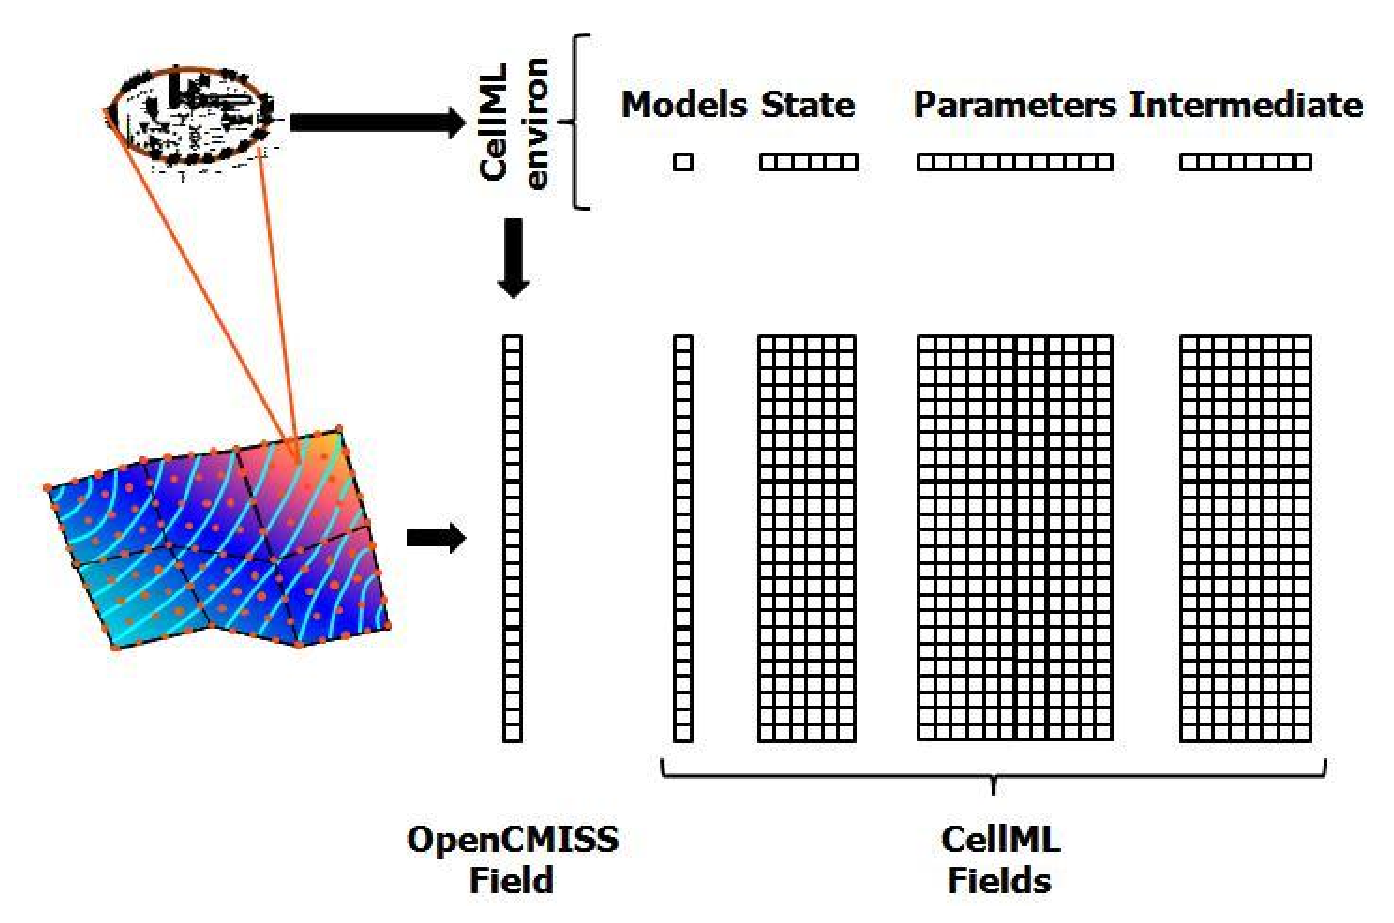
\includegraphics[width=0.7\textwidth]{figs/Modules/cellml_interface.eps}
\caption{Diagram showing \emph{OpenCMISS} field and \emph{CellML} fields.}
\label{cellml_interface}
\end{figure}


\section{Library: \emph{FieldML}}
\label{sec:fieldml}

\emph{FieldML} (Field modelling Markup Language) is used to read/write the
field descriptions in \emph{OpenCMISS}. \emph{FieldML} is a declarative 
language for building hierarchical models represented by generalized 
mathematical fields. It is intended as a framework for modelling software 
development and model interchange for bioengineering and general 
engineering analysis communities. To date \emph{FieldML} has not been 
fully integrated into \emph{OpenCMISS} and remains a project under 
development.


\section{Module: \emph{base\_routines}}
\label{sec:baseroutines}

This module contains the error handling, diagnostic, timing routines, and 
the \emph{ENTERS} and \emph{EXITS} routines. The \emph{ENTERS} and 
\emph{EXITS} routines use the global \emph{ROUTINE\_STACK} object to store 
a list stack of the routine passed through during execution. This is used 
for the diagnostics and for display when a program fails. Also attached to 
this object is the \emph{CPU\_TIMING} routines that record the execution time 
between the \emph{ENTERS} and \emph{EXITS} calls in a subroutine.The global 
boolean \emph{TIMING} variable is used to switch the timing on, and the global 
boolean \emph{DIAG} variable is used to switch the diagnostics on. 

The \emph{command} file, \emph{learn} file and \emph{echo} files are legacy 
files and their use is not implemented.


\section{Module: \emph{basis\_routines}}
\label{sec:basisroutines}

This module contains the routines for defining the basis functions and element 
topological properties (for example local and global node numbering). The basis 
function is the key item to specify the field approximation/interpolation and 
the linking of nodes and elements to form a mesh. The node position index 
serves as a means of identifying the position of the node within the basis.

A basis function can either be Lagrange-Hermite tensor product (LHTP) type or 
simplex type. For the LHTP basis type, linear lagrange, quadratic lagrange, 
cubic lagrange, and cubic hermite are available in \emph{OpenCMISS}. For the 
simplex basis type: linear, quadratic, and cubic lagrange are available. In 
\emph{OpenCMISS} Gaussian quadrature can integrate from 1st to 5th order 
(currently 3rd order for lines at the moment). 

Only one basis function can be defined per basis object. \emph{OpenCMISS} does 
allow a mix of different interpolations for different $\xi$ directions, though 
only for a mixture of LHTP basis types. 

In \emph{OpenCMISS} specifying a basis function automatically generates all the 
necessary line and face basis functions as sub-bases of the basis function. 
Faces and lines in an element have both local numbers and global numbers, the 
local numbering scheme for \emph{Hex} and \emph{Tet} elements is shown in the 
diagrams below. For LHTP type the direction of a face in \emph{OpenCMISS} is
defined by the normal to the face (for $3D$) or line (for $2D$), for simplex 
types it is defined as the tangent from the point opposite to the face (for 
$3D$) or the line (for $2D$) running out through the face/line at 
right-angles (see diagrams).

The simplex type basis in \emph{OpenCMISS} uses the bary-centric coordinate 
system of area coordinates. The area coordinate is the ratio of the covered 
area to the uncovered area. The area of a triangle is defined with three 
coordinates: $L1$, $L2$ and $L3$. The definition of area coordinates is such 
that the sum of the coordinates equals $1$, this allows only $L1$ and $L2$ to 
be used and $L3$ dropped. Simplex type basis functions can have line,
triangular and tetrahedral elements. 

There are two variables in \emph{OpenCMISS} for the number of $\xi$: \\
\emph{NUMBER\_OF\_XI\_COORDINATES} which is used for the number of actual 
$\xi$ coordinates that the user can specify, this is the topological system, 
and \emph{NUMBER\_OF\_XI} which is used for the number of independent $\xi$ 
coordinates. If it is a two dimension manifold then this variable will be 
two. This is primary for bary-centric coordinate system where we can have 
more than one parametric coordinate.

The basis functions handle collapsed bases, a collapsed basis (where there are 
two or more nodes in the same location) is called a degenerate basis. Both $2D$ 
elements and $3D$ elements can be collapsed. They can be collapsed in any one 
direction or in two directions, and are defined by the direction of collapse 
and the end of collapse, either the $\xi=0$ end or $\xi=1$ end. Simplex
elements cannot be collapsed. The collapse is defined by the 
\emph{xi\_collapsed} parameter, this has three possible states: 
\emph{collapsed\_at\_xi1}, \emph{collapsed\_at\_xi0} and 
\emph{not\_collapsed}, these define the direction and point of collapse. In
nodal interpolation, the nodes of the collapsed line or face are bunched into 
a point (for the collapsed of a line) or line (for the collapsed of a face).
When an object collapsed one end loses it's derivative. This is defined in 
OpenCMISS using the \emph{BASIS\_QUADRATIC1\_HERMITE\_INTERPOLATION} parameter
that defines that for a line there is no derivative at the $\xi=0$ end, and 
the  \emph{BASIS\_QUADRATIC2\_HERMITE\_INTERPOLATION} parameter that defines 
that there is no derivative at the $\xi=1$ end.

The serendipity (where there is no central point in a face), fourier and
singular interpolation schemes have not currently been implemented in 
\emph{OpenCMISS}, although place holders exists for their use.

The following three parameters have not been currently enabled in OpenCMISS: 
\emph{BASIS\_LOW\_QUADRATURE\_SCHEME}, \emph{BASIS\_MID\_QUADRATURE\_SCHEME},
\emph{BASIS\_HIGH\_QUADRATURE\_SCHEME} these are for use in the implementation
of boundary elements.

In addition to the basis functions described above, there are also face gauss 
basis functions the face gauss basis functions are $3D$ objects allowing the 
calculation of the derivative in the third dimension at the face.

In this module the node numbering of the elements is set. The node 
numbering is as follows:

\begin{figure}
\centering
      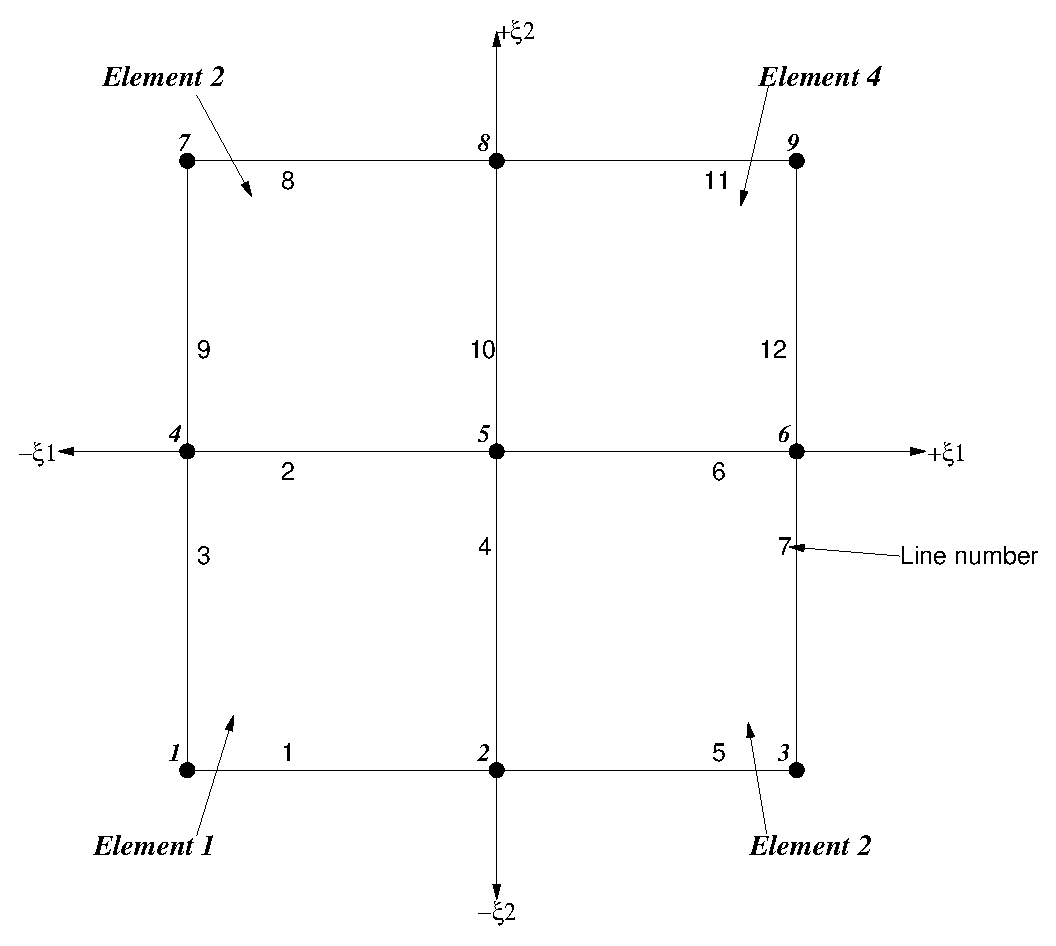
\includegraphics[width=0.6\textwidth]{figs/Modules/2D_linear.eps}
\caption{Diagram showing node numbering, line numbering and $\xi$ directions 
for a 2D arrangement of four elements with linear interpolation.}
\label{2D_linear}
\end{figure}

\begin{figure}
\centering
      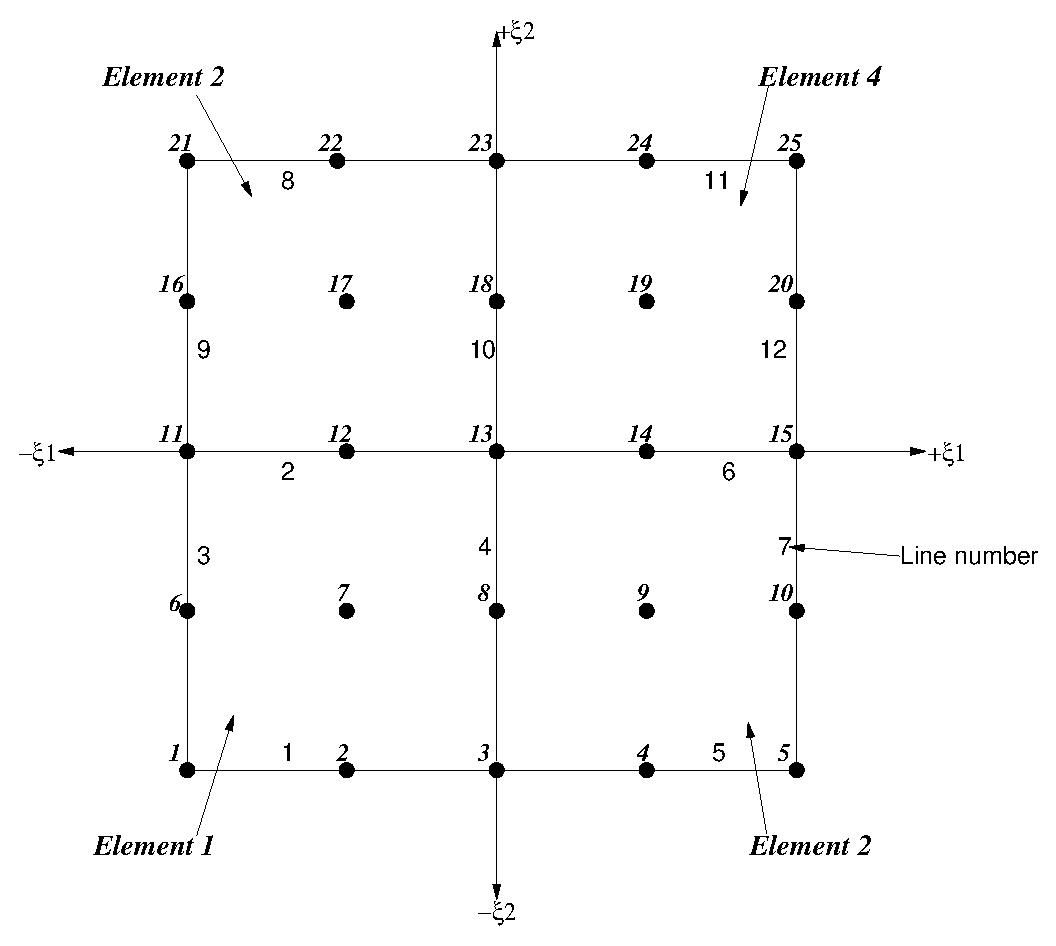
\includegraphics[width=0.6\textwidth]{figs/Modules/2D_quadratic.eps}
\caption{Diagram showing node numbering, line numbering and $\xi$ directions 
for a 2D arrangement of four elements with quadratic interpolation.}
\label{2D_quadratic}
\end{figure}

\begin{figure}
\centering
      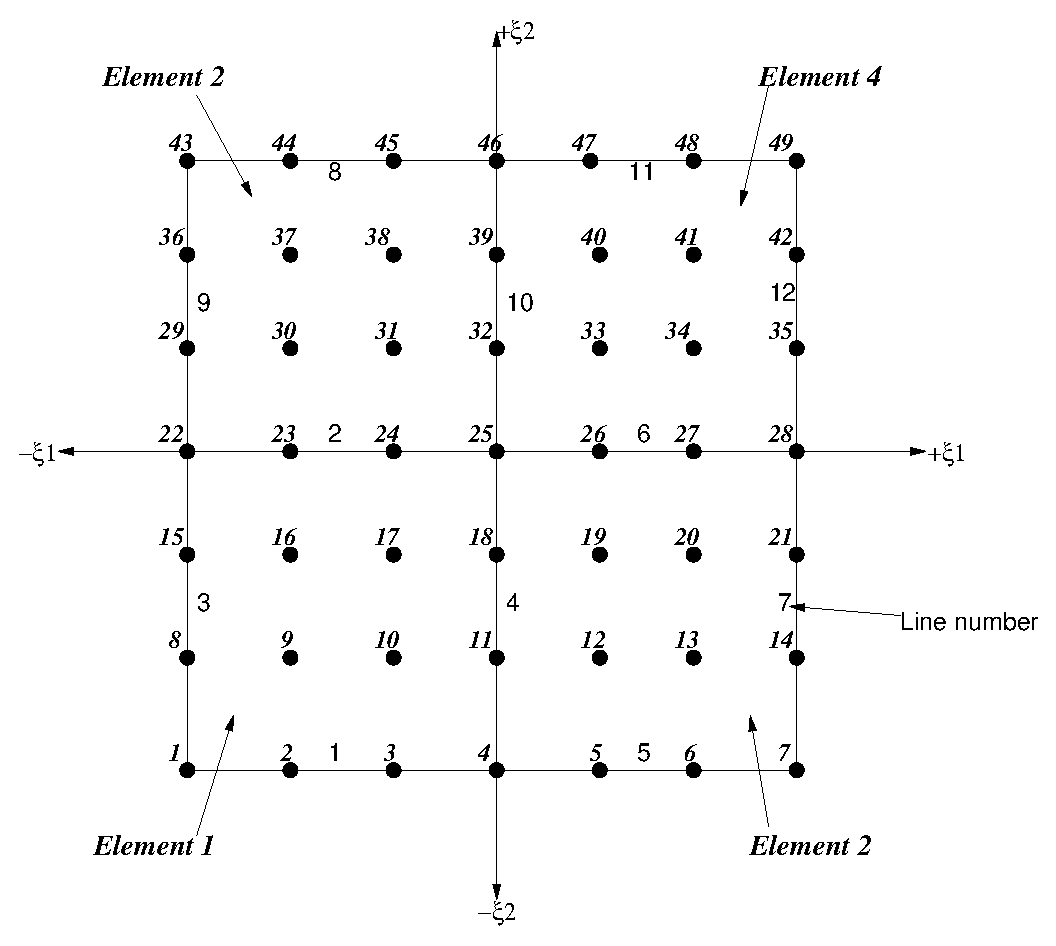
\includegraphics[width=0.6\textwidth]{figs/Modules/2D_cubic.eps}
\caption{Diagram showing node numbering, line numbering and $\xi$ directions 
for a 2D arrangement of four elements with cubic interpolation.}
\label{2D_cubic}
\end{figure}

\begin{figure}
\centering
      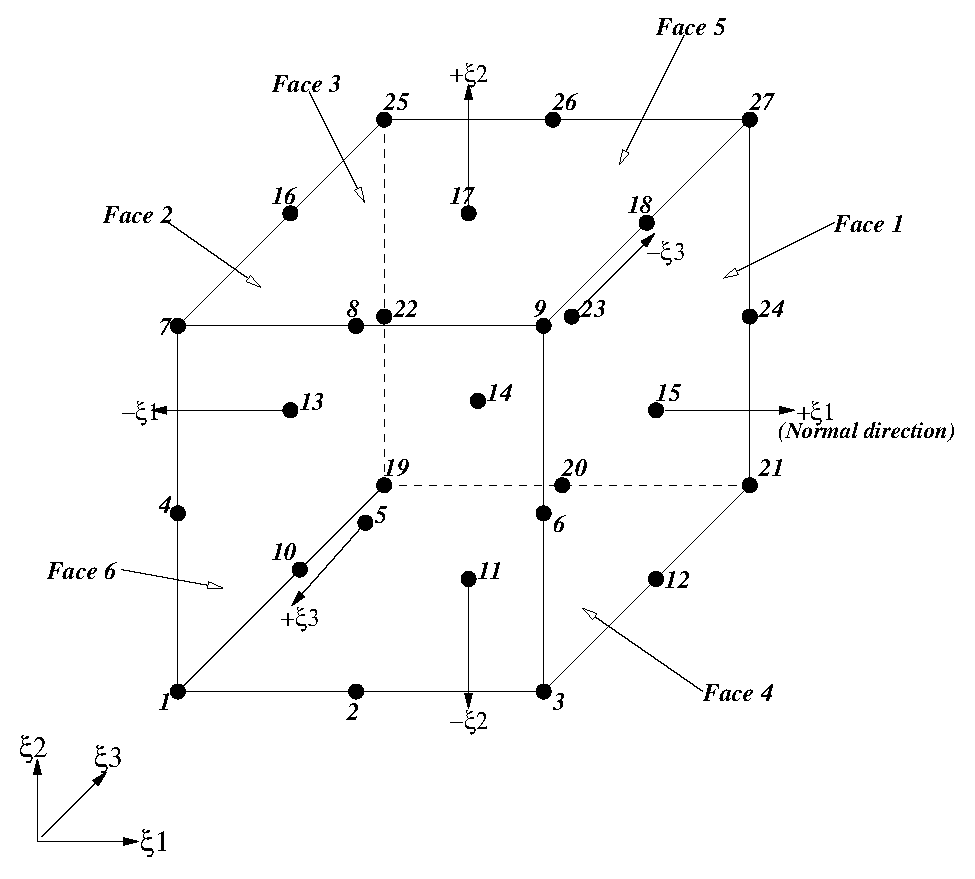
\includegraphics[width=0.6\textwidth]{figs/Modules/cube.eps}
\caption{Diagram showing node numbering, line numbering and $\xi$ directions 
for a single 3D element with quadratic interpolation.}
\label{cube}
\end{figure}

\begin{figure}
\centering
      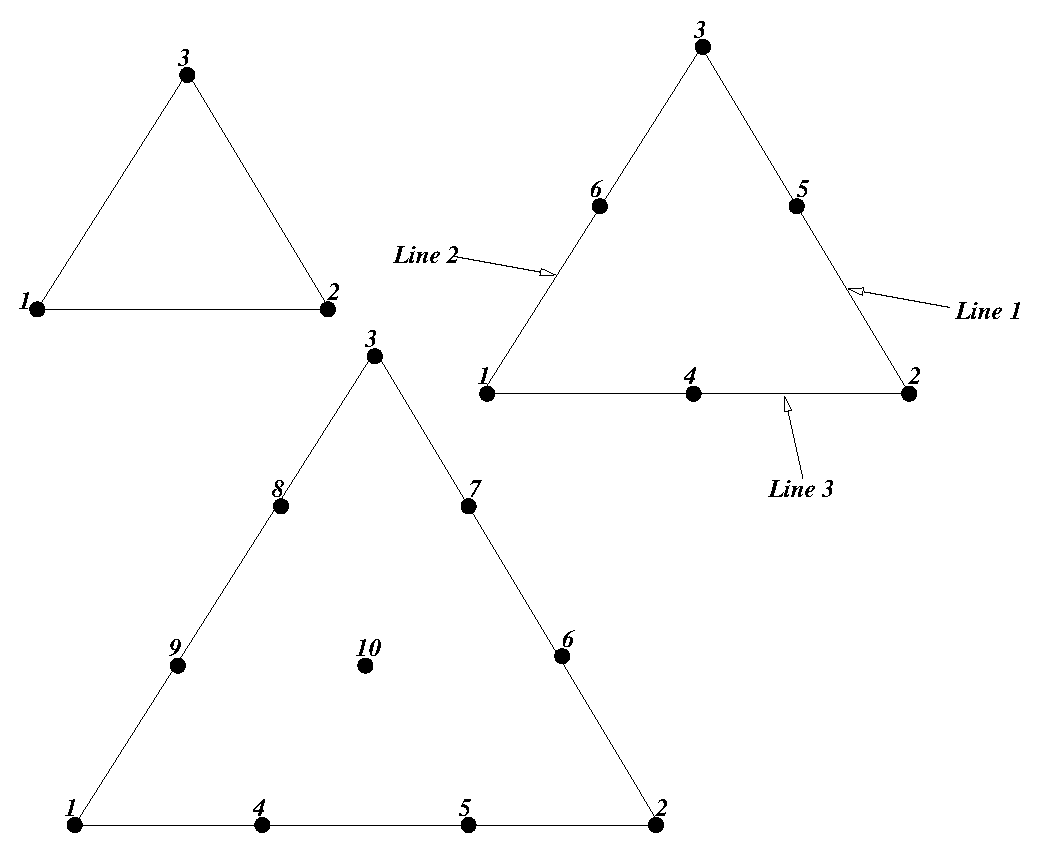
\includegraphics[width=0.6\textwidth]{figs/Modules/tri_elements.eps}
\caption{Diagram showing node and line numbering for single 2D tri elements 
with linear (top left), quadratic (top right) and cubic (bottom) 
interpolation.}
\label{tri_elements}
\end{figure}

\begin{figure}
\centering
      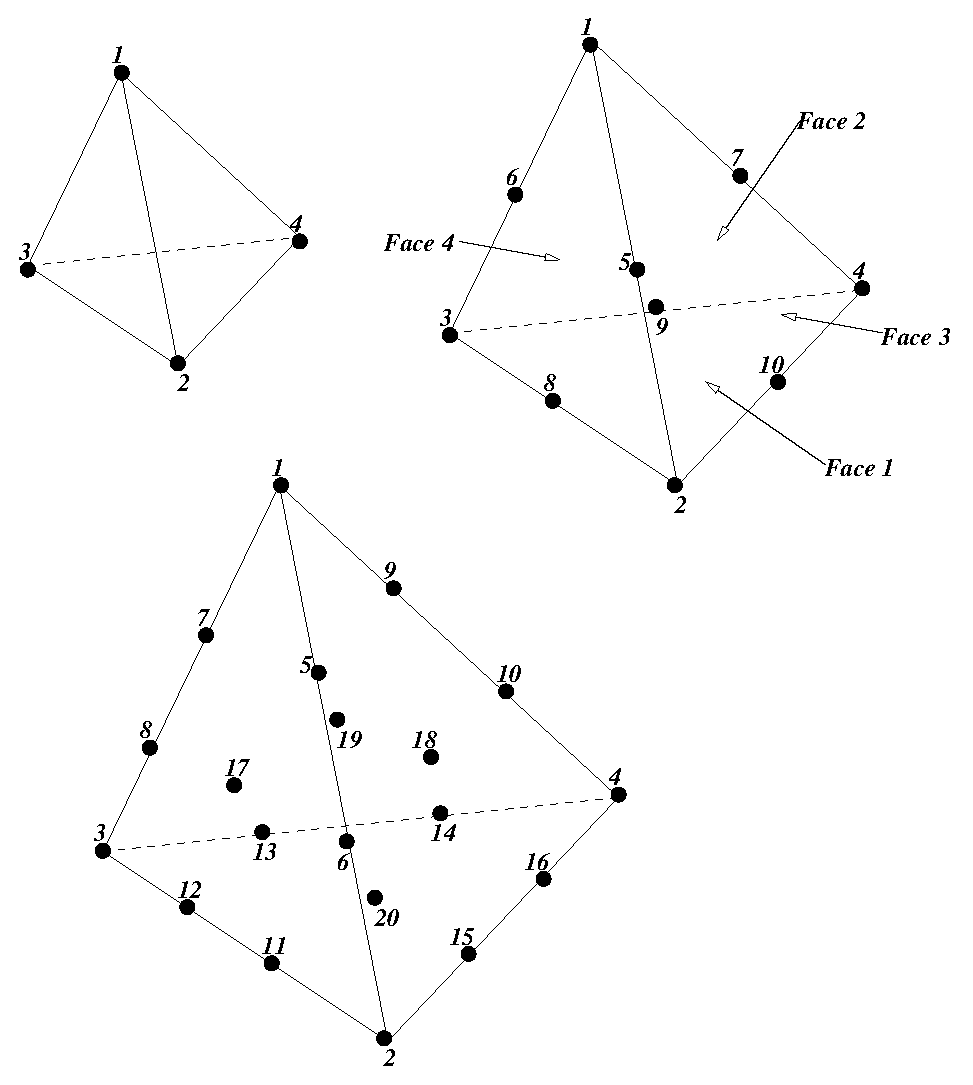
\includegraphics[width=0.6\textwidth]{figs/Modules/tet_elements.eps}
\caption{Diagram showing node and line numbering for single 3D tet elements 
with linear (top left), quadratic (top right) and cubic (bottom) 
interpolation.}
\label{tet_elements}
\end{figure}

\begin{figure}
\centering
      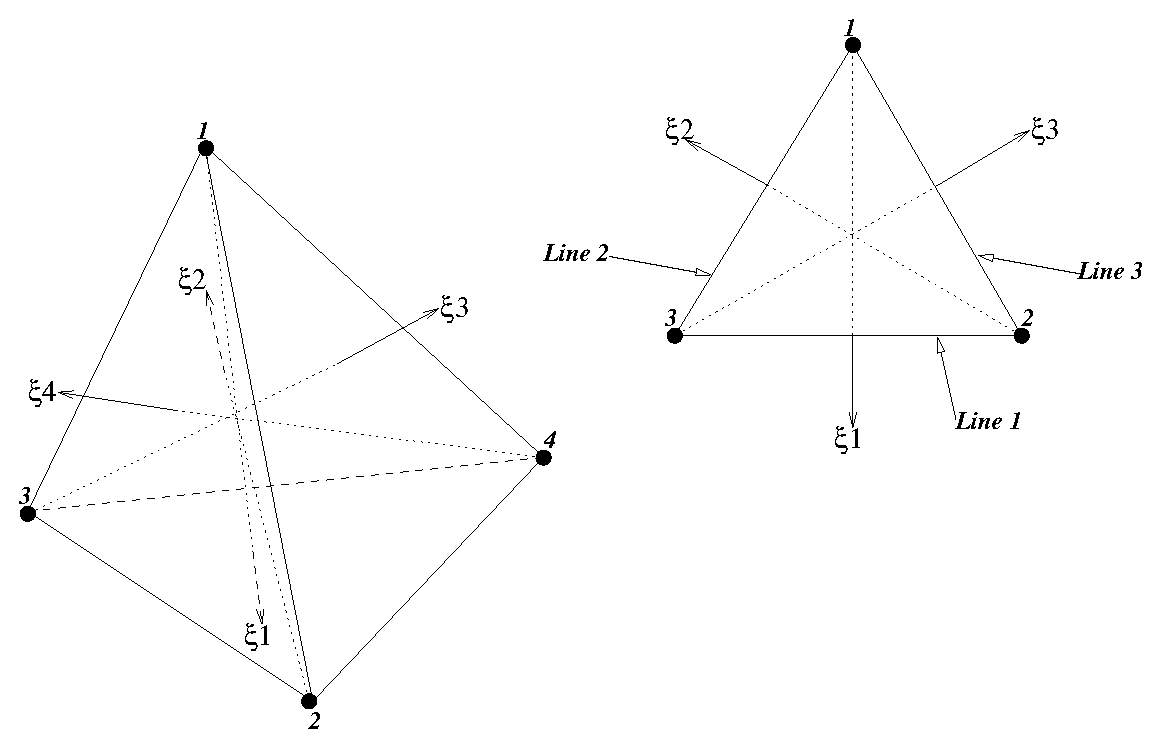
\includegraphics[width=0.7\textwidth]{figs/Modules/tet_normals.eps}
\caption{Diagram showing $\xi$ directions for a tet element (left) and  
a tri element (right), both with linear interpolation.}
\label{tet_normals}
\end{figure}

\begin{figure}
\centering
      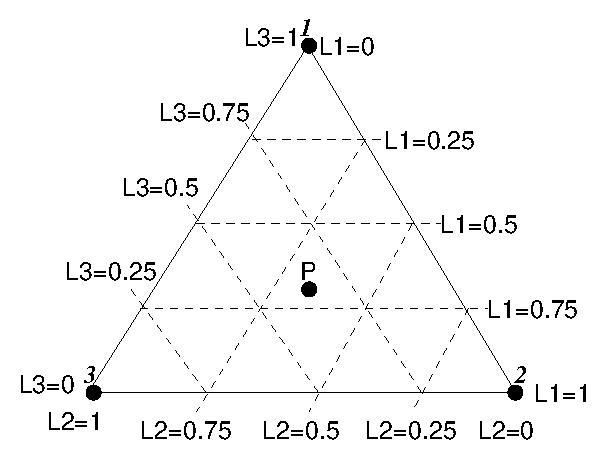
\includegraphics[width=0.6\textwidth]{figs/Modules/Tri_area_coordinates.eps}
\caption{Diagram showing $L1$, $L2$ and $L3$ area coordinates for a 2D 
tri element.}
\label{Tri_area_coordinates}
\end{figure}


\section{Module: \emph{boundary\_condition\_routines}} 
\label{sec:boundaryconditionroutines}

There are two basic types of boundary condition: \emph{fixed} and 
\emph{free}. The type is the status of the value held at the dof (the 
dof at the boundary), if the type is fixed the value of the dof is 
set and it is removed from the main problem calculation, and if the type 
is free the value of the dof is included and calculated in the main 
problem calculation. In the \emph{fixed} type there are a number of 
sub-types: \emph{Neumann}, \emph{Dirichlet} and \emph{Incremented} 
(boundary dof values change with time). The \emph{Neumann} boundary 
conditions operate on the \emph{RHS}, and the \emph{Dirichlet} boundary 
conditions operate on the \emph{LHS}. 

The \emph{Dirichlet} boundary condition applies to a dof, if a dof is 
set to fixed (that is the boundary condition on the dof is fixed) and 
if all other entries in the row of the solver matrix $A$ correspond to 
fixed dofs, then the Dirichlet condition applies and the row and column 
in the solver matrix $A$ in which the value that corresponds to the dof 
resides, can be removed. The \emph{Dirichlet} boundary conditions use 
a linked-list with the matrix sparsity pattern, more details are provided 
in the theory section on the \emph{Dirichlet} boundary conditions. Also 
further details on the \emph{Neumann} boundary conditions are provided 
in the theory section.

To date the type of boundary condition is not clearly delinated from the 
sub-type, this needs to be clarified in the future. 


\section{Module: \emph{classical\_field\_routines}}
\label{sec:classicalfieldroutines}

This module is the top level module to the generic physics modules (classical 
field type), it contains the calling routines for the generic physics routines. 
The classical field type includes the physics types of: \emph{Advection
Diffusion}, \emph{Biharmonic}, \emph{Diffusion}, \emph{Hamilton Jacobi}, 
\emph{Helmholtz}, \emph{Laplace}, \emph{Poisson}, \emph{Reaction Diffusion} 
and \emph{Wave}. \emph{Biharmonic}, \emph{Reaction Diffusion} and \emph{Wave} 
are not currently implemented.


\section{Module: \emph{cmiss}}
\label{sec:cmiss}

This module contains the top level initialise and finalise routines that are
used by all modules and example files.


\section{Module: \emph{cmiss\_petsc} \& \emph{cmiss\_parmetis}}
\label{sec:cmisspetscandcmissparmetis}

The binding for \emph{OpenCMISS} to \emph{PETSc} and \emph{ParMETIS}, 
are contained in this module, The routines in this module translate 
required and returned types, and act as buffers with error codes for the 
\emph{OpenCMISS} calling routines.


\section{Module: \emph{control\_loop\_routines}}
\label{sec:controllooproutines}

Control loops describe the workflow that will be used to solve a problem.
A control loop has a pre-control routine and a post-control routine, these 
contain actions to be performed before (pre-control) or after (post-control) 
the control loop has completed an iteration. This allows for problem specific 
actions to be performed, for example the time varying boundary conditions or 
the writing out to a file of time dependent solutions (this is work in
progress).

Control loops are either be: simple, executing once; iterative, executing a
number of specified times (with additional parameters within this loop i.e., 
a control variable of a start value plus an increment); or conditional, the 
loop executes until a condition is met (for example a convergence condition).

Each control loop has a number of sub loops, if a control loop has no sub loops 
it can have a number of solvers. Each solver deals with a particular numerical 
problem solver.

\begin{figure}
\centering
      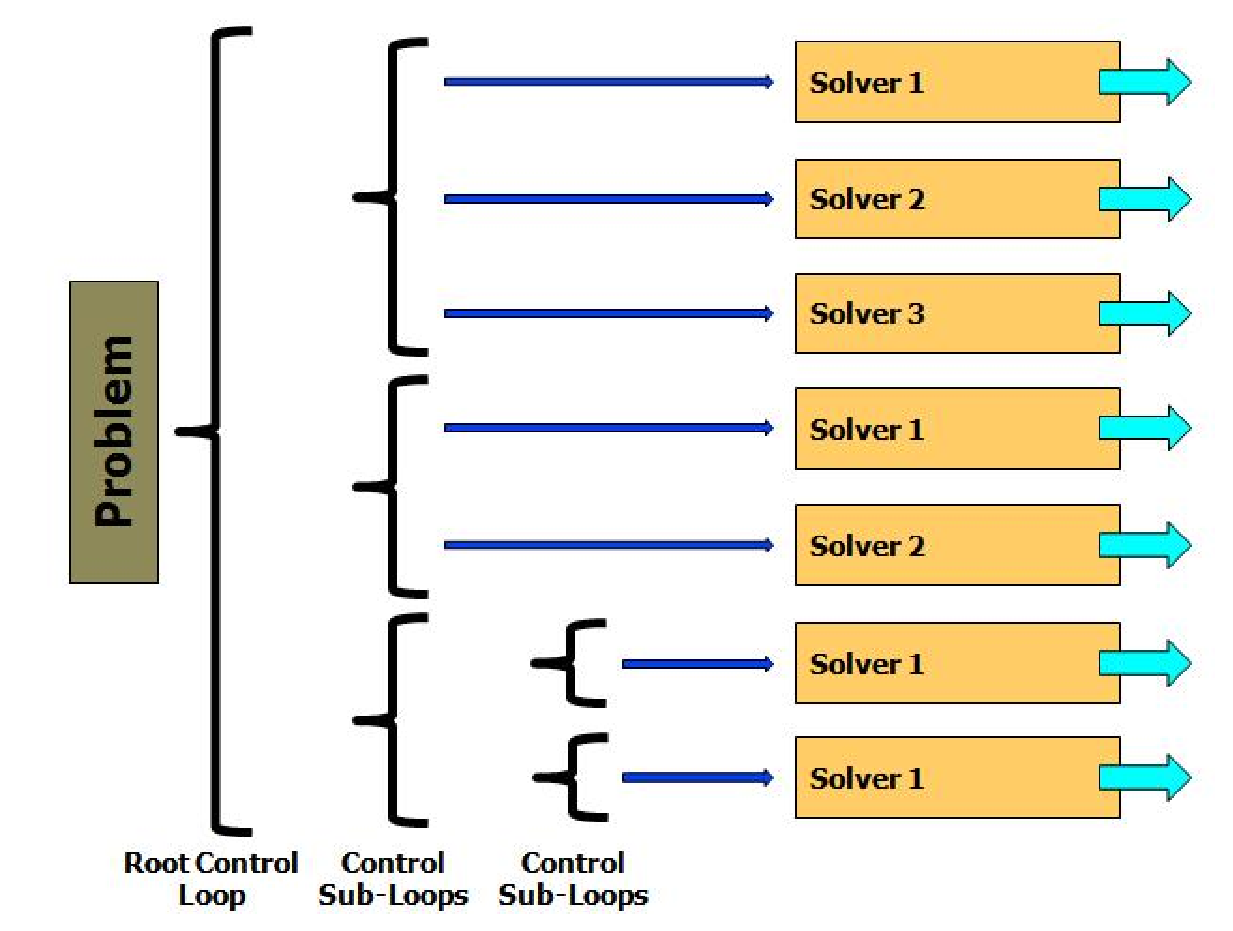
\includegraphics[width=0.6\textwidth]{figs/Modules/control_loops.eps}
\caption{Diagram showing sub-control loops and associated solvers within a 
control loop.}
\label{control_loops}
\end{figure}



\section{Module: \emph{coordinate\_routines}}
\label{sec:coordinateroutines}

A coordinate system is a system for assigning an $n$-tuple of numbers or
scalars to each point in an $n$-dimensional space. It anchors the regions 
within the real world. \emph{OpenCMISS} has been designed to support a number 
of different coordinate systems: rectangular cartesian, cylindrical polar, 
spherical polar, prolate spheroidal or oblate spheroidal. Currently only the 
rectangular cartesian (RC) coordinate system has been fully implemented. 
There are however routines for the conversion of cylindrical polar, spherical 
polar, prolate spheroidal and oblate spheroidal coordinates to RC coordinates.

A coordinate system in \emph{OpenCMISS} is defined with respect to the parent 
coordinate system, whilst the parent coordinate system itself is defined with 
respect to the RC coordinate system. The parent coordinate system is the top 
coordinate system in a region. Only one coordinate system is allowed to be 
attached to a coordinate system object and only one coordinate system is 
allowed per region. The global coordinate system is the world coordinate 
system, and is the parent coordinate system of all the regions. 


\section{Module: \emph{data\_point\_routines} \&  \\ 
\emph{data\_projection\_routines}}
\label{sec:dataprojectionroutines}

The data projection routines enable the fitting of experimentally gathered 
data to a field. In \emph{OpenCMISS} the data is approximised to a linear 
problem, then stored as a data field, and solved as a linear function. The 
data projection routines calculate the projection of the data points to the 
elements in the mesh. Enabling these data points to be decomposed as the 
elements are decomposed during the execution of the program. 

Geometric fields are ordinarily worked out after the geometric position is 
assigned, however in \emph{OpenCMISS} we cannot do this, so in order to 
construct the data field from the data, we assign a starting guess of the 
centroid of candidate element to a data point, then we use Newton's method to 
find the closest face/line and $1D$, $2D$ or $3D$ element to the data point, 
enabling the position of the data point to be set and stored in the data field. 
The number of dofs in the data field is determined by the number of data points 
to which the field is fit.

Future work in these routines include the wrapping of the projection method
as a solver.


\section{Module: \emph{distributed\_matrix\_vector}}
\label{sec:distributedmatrixvector}

The routines in this module set up the matrices and vectors for the problem 
and handle the communication of the changes in the values in the matrices and 
vectors. With multiple processors (domains) the routines handle the splitting 
of the matrices and vectors by rows allowing the matrices and vectors to be
distributed evenly across processors. 

The routines allow different solver library to be used with the matrices and 
vectors; with either internal or external solver libraries.

The override matrix/vector allow the overriding of the \emph{PETSc}
matrix/vector with an incoming matrix/vector from \emph{PETSc}.

The receive buffer and the send buffer handle the communication between the 
domains of the ghost values.


\section{Module: \emph{domain\_mappings}} 
\label{sec:domainmappings}

These routines set what the local and global domain numbers are, and what 
local numbers and global numbers need to be exchanged. \\
Each domain stores the domain information for the relevant mesh component. \\
The first pass does the local ones and second pass does the ghost ones. \\
Calculates global to local.


\section{Module: \emph{equations\_mapping\_routines}}
\label{sec:equationsmappingroutines}

The routines in this module are used to calculate how the field variables 
are mapped on to equations matrices and vectors.


\section{Module: \emph{equations\_matrices\_routines}}
\label{sec:equationsmatricesroutines}

The routines in this module handle the creation, deletion of equations 
matrices.


\section{Module: \emph{equations\_routines}}
\label{sec:equationsroutines}

Equations hold the matrices and mapping information. The field variable 
to matrix mappings maps each field variable onto the equations matrices or 
\emph{RHS} vector.


\section{Module: \emph{equations\_set\_constants}}
\label{sec:equationssetconstants}

This module is used to store the constants used by routines in the \\
\emph{equations\_set\_routines} module they are separated out from 
other constants to avoid circular model dependency.


\section{Module: \emph{equations\_set\_routines}}
\label{sec:equationssetroutines}

Equations set objects are the containers for containing information on 
particular physics setup, they are the fundamental objects in 
\emph{OpenCMISS} that are used to encapsulate a single physics. In 
\emph{OpenCMISS} the solvers require equations sets.

Multiple equations sets are used for problems with multiple physics 
(\emph{classes}), with coupling required between them, this is 
dependent upon the problem. A single physics problem has only one 
equations set per region. For a single physics example (for example: 
\emph{Laplace}) operating across a number of regions, there will need 
to be one equations set per region over which the physics operates.

To set up an equations set object the user needs to first create fields and
attach these to the equations set object, otherwise default fields will be 
attached to the equations set object.

An equations set object has a number of possible parts: a geometric field, 
a fibre field, an independent field, a dependent field, a material field, a 
source field and the equation. The geometric field and the dependent field 
are the minimum fields attached to the equations set object.

The equations object (attached to the equations set object) represents the 
numerically discrete approximation of the problem over the region in terms of 
the matrices and vectors of the governing equation of the problem. 
\emph{OpenCMISS} is designed to generate equations sets with a number of 
equation matrices. Each equations object can have a different solution 
techniques, e.g. FEM, BEM, FD or GFEM. 

A special case is the FMM (Fast Marching Method) which does not use an 
equation. So this type will use an equations set, but the equations set for 
FMM will not have any equations associated with it. 

In parallel the same equations set exists across all the processors (the 
domains), however both the fields and equations are distributed across the 
processors. The splitting of the equations matrix is: rows are locally number, 
whilst columns are globally numbered. \emph{PETSc} requires global numbers.


\section{Module: \emph{field\_routines}}
\label{sec:fieldroutines}

Data in \emph{OpenCMISS} is stored in the form of fields, fields are the 
central object for storing information and framing the problem. Fields are 
composed of: variables, components, dofs and parameters. The numerical 
values in a field are stored in the parameters.

Each field can have multiple variables. The $u$ variable type represents 
the \emph{LHS} and the \emph{deludeln} ($\partial{u}/\partial{n}$) variable 
the \emph{RHS} of the equation. There is also a \emph{deludelt} 
($\partial{u}/\partial{t}$) variable available to be used depending upon 
the physics being solved. The user must specify in the example call program 
which variables to have attached to a field, the minimum number of variables 
is one. Multiple $u$ and \emph{deludeln} ($\partial{u}/\partial{n}$) 
variables are available for use in volume coupling, with each set of $u$ 
and \emph{deludeln} ($\partial{u}/\partial{n}$) variables representing a 
different physics in the region. The variable types are labels. 

Variables are composed of components, for example the components of velocity 
in the $x$, $y$ and $z$ direction: $u$, $v$ and $w$, would be the components 
of one variable the $u$ variable. Any number of components can be defined to a
variable (with a minimum of one component). 

A field is defined on a decomposed mesh. Each component of a field is defined 
on a decomposed mesh component.

Components contain the dofs. Different variables (and components) in a given 
field can have different numbers of dofs, also at the field level each field 
in a problem can each have a different number of dofs. The dofs of the 
components in a variable are stored together in a single vector. There are 
two options for the organisation of the dofs in a component: separated dof 
order and contiguous dof order. 

In separated dof ordering all dofs of each component are stored together.
In contiguous dof ordering all dofs of a parameter (for example a node in 
node based interpolation) are stored together. Continguous dof ordering can 
only be chosen if each of the components have the same interpolation and dof 
structure, hence the default is separate dof ordering.

In terms of the storage of data in memory, contiguous blocks of memory are 
preferred over distributed blocks of data in the memory, this has been central 
to the design of OpenCMISS. This has been implemented with the storage of 
components (and subsequently dofs) as a single vector, rather than the storage 
of a separate block for each component.

The \emph{dof type} defines what sort of dofs are in the field, essentially
where the dofs are positioned in the field, either as constant dofs (only one 
set of dofs for the field), element dofs (one set of dofs per element), node 
dofs (one set of dofs per node), grid point dofs (one set of dofs per grid point), 
or gauss point dofs (one set of dofs per gauss point). A set of dofs consists of 
a dof for each defined component for the variable, and a dof for each derivative 
(derivatives are used for Cubic Hermite basis functions).

There are three types of dof numbering: local, ghost and global. The global dof 
numbering refers to the numbering of all dofs in the mesh. The local dof
numbering is the dof numbers of the dofs in the local domain. The ghost dof 
numbering is the nearest dof number 

A domain is the decomposed problem space assigned to the individual processor 
following the decomposition of the problem over a number of processors. There
is one domain per processor. 

The \emph{field mapping calculate} routine sets up the local and ghost dof
numbering scheme for the domain and the mapping of these local dofs numbers 
to the global dofs.

The dofs (indexed by $ny$) are organised in a component with the local dofs
first followed by the ghost dofs. This allows looping, when required, to be made 
only over the local dofs. The ordering of local and ghost dofs in a component is
made in the \emph{field mappings calculate} routine.

The \emph{field mappings calculate} routine operates with the following steps:

\begin{enumerate}
 \item Calculate how many dofs and parameters
 \item Calculate the parameter to dof mapping
 \item Calculate the dof to parameter mapping
 \item Calculate the global dof to local dof mapping
\end{enumerate}

The \emph{field mappings calculate} routine does two sweeps, the first to
calculate how many values are required, and the second to allocate the arrays.

The labeling of variables containing collections of dofs are: if the variable 
name contains \emph{number\_of\_local} then this is the per domain dofs, if it 
contains \emph{total} then this refers to local and ghost dofs, or if it 
contains \emph{global} then this refers to all local and ghost dofs across all 
elements (the total number of undistributed items).

\begin{figure}
\centering
      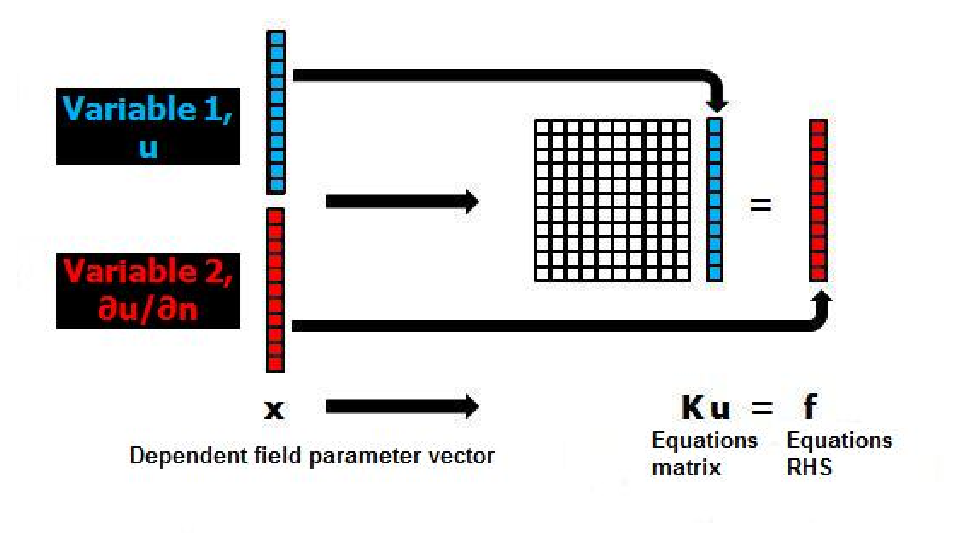
\includegraphics[width=0.7\textwidth]{figs/Modules/variable_mapping_1.eps}
\caption{Diagram showing showing variable mappings.}
\label{variable_mapping_1}
\end{figure}

\begin{figure}
\centering
      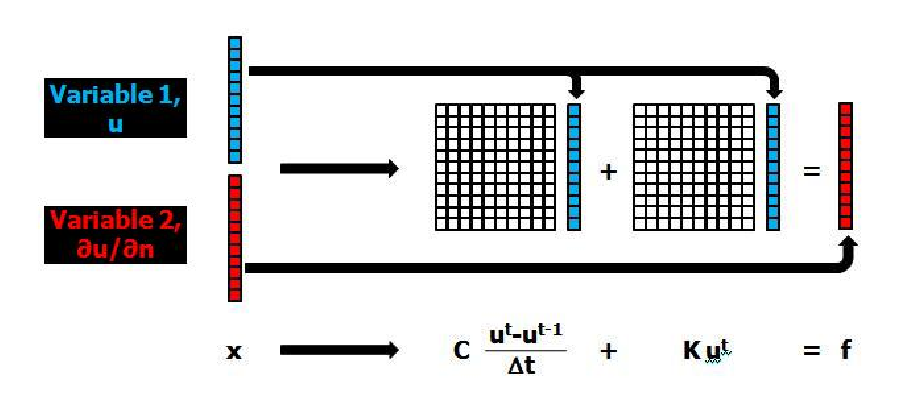
\includegraphics[width=0.7\textwidth]{figs/Modules/variable_mapping_2.eps}
\caption{Diagram showing showing variable mappings.}
\label{variable_mapping_2}
\end{figure}

\begin{figure}
\centering
      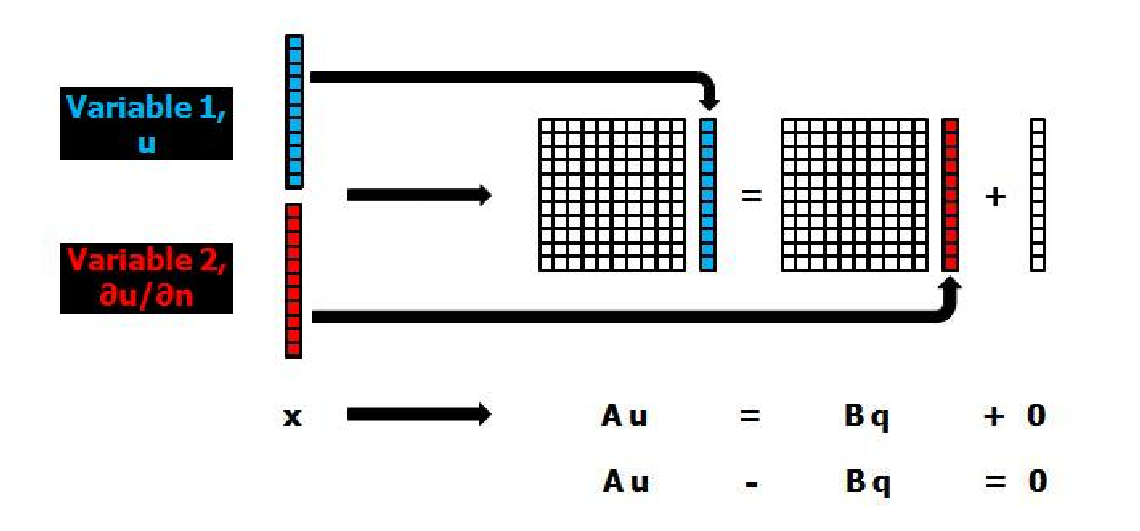
\includegraphics[width=0.7\textwidth]{figs/Modules/variable_mapping_3.eps}
\caption{Diagram showing showing variable mappings.}
\label{variable_mapping_3}
\end{figure}


\section{Module: \emph{finite\_element\_routines}}
\label{sec:finiteelementroutines}

This module is not currently used in \emph{OpenCMISS}.


\section{Module: \emph{fitting\_routines}}
\label{sec:fittingroutines}

The fitting routines project/fit material data onto some field interpolation.
The routines take as input given material data at the interpolation points (the
gauss points) and project the data onto the desired field interpolation to give
a material field interpolation. It reduces the vector down to the Galerkin
space, it is the minimum projection, the closest one can get to representing a 
vector on a space using available basis functions. It builds a projection matrix 
(\emph{LHS}) and a projection vector (\emph{RHS}). The fitting object itself' 
is an equations set object.


\section{Module: \emph{generated\_mesh\_routines}}
\label{sec:generatedmeshroutines}

The routines in this module generate the mesh required by the problem, the 
routines call the mesh topology element generation routines. In 
\emph{OpenCMISS} currently either rectangular, cylindrical and ellipsoidal 
meshes can be generated with these routines.

The extent of the generated mesh is defined in the example program by the 
\emph{width}, \emph{length} and \emph{height} parameters, the size of the 
individual elements in the generated mesh is defined as the division of each 
of these parameters by the total number of elements.

\emph{OpenCMISS} allows multiple generated meshes to be assigned to one region 
(indexed by a global number), with only one generated mesh per generated mesh 
object. Interfaces act like regions, a generated mesh can be on a region or an
interface. The generated mesh uses the basis object.

The completed generated mesh object becomes the mesh object.


\section{Interface modules}
\label{sec:interfacemodules}

This module covers the surface coupling routines. These routines allow the 
mapping/coupling of two meshes between two different regions on a shared
surface. Both meshes are defined with respect to the shared surface (the 
interface). The surface coupling routines allow the coupling of two regions 
of two different interpolation types. 

An interface object is equivalent to, and operates at the same level as 
the region type object. The interface object provides flexibility outside 
of the normal regions/equations/equations sets structures, enabling 
independent editing of the interface data structures.

An interface condition is an object that is similar to an equations set 
object. 

There are a number of operators and methods available to determine the 
coupling between the regions. The operator is dependent upon the type of 
equation being coupled, and the method refers to the mathematical method of 
coupling.

Surface coupling to date has been implemented and tested for \emph{Hex} 
elements, it has been implemented for both \emph{Tet} elements, and mixtures 
of \emph{Hex} and \emph{Tet} elements, though to date remains to be fully 
tested for both of these.

Surface coupling is not currently working in parallel, this remains 
\emph{work in progress}, when complete, both coupled regions will 
parallelise in a similar fashion.

\begin{figure}
\centering
      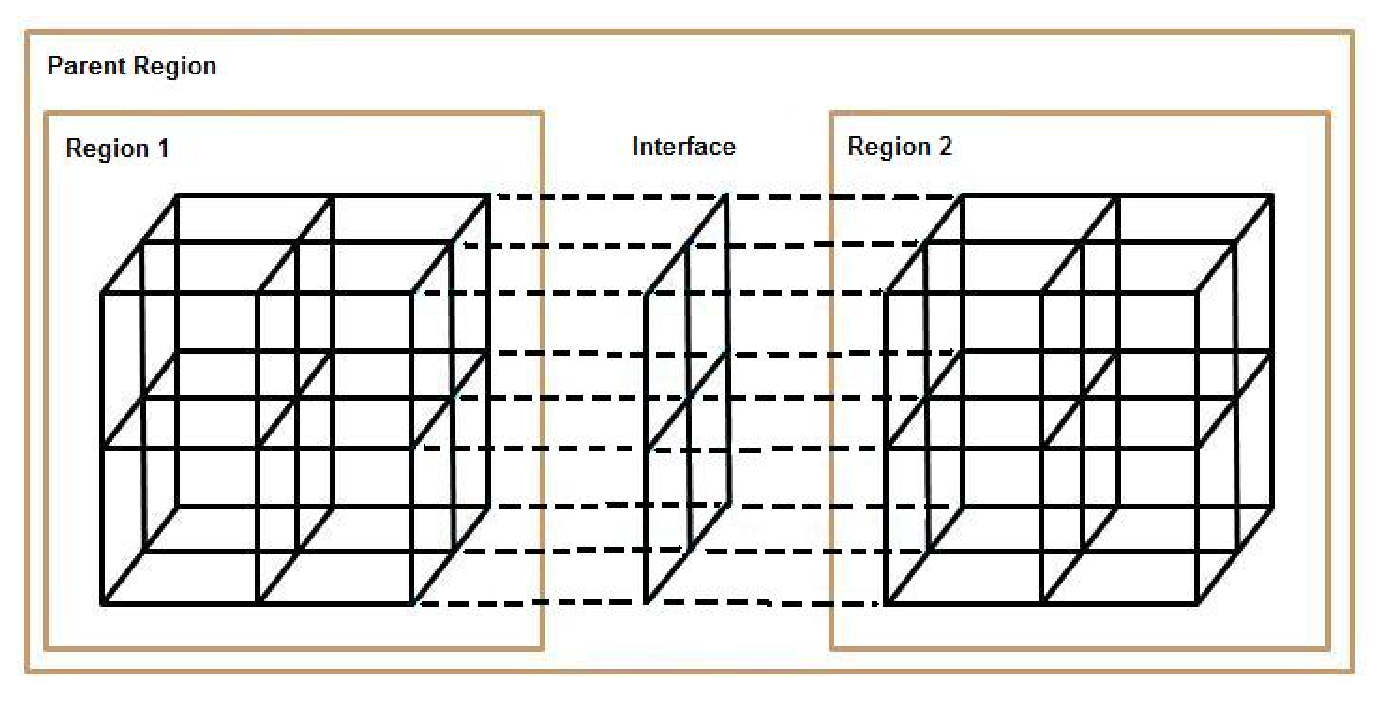
\includegraphics[width=0.7\textwidth]{figs/Modules/interfaces.eps}
\caption{Diagram showing the interface between two regions.}
\label{Interfaces}
\end{figure}



\section{Module: \emph{kinds}}
\label{sec:kinds}

This module handles the different data types available in \emph{OpenCMISS}: 
\emph{\_DP} (double precision), \emph{\_INTG} (integer), \emph{\_SP} (single 
precision) or \emph{\_L} (logical). The '\emph{\_}' (a Fortran source term) 
means a different \emph{kind} in Fortran. In addition, a number of kinds 
are defined preceded by \emph{CMISS} these are equal to a corresponding 
kind, for example: \emph{\_CMISSDP} is equal to \emph{\_DP}. 


\section{Module: \emph{lists}}
\label{sec:lists}

This module contains the routines for lists, lists are data structures that 
allows the listing of items, their ordering and de-duplication.


\section{Module: \emph{matrix\_vector}}
\label{sec:matrixvector}

The routines in this module are a subset of the distributed matrix routines, 
and are only for routines that operate on an individual domain/processor.

Matrices are stored as a combination of three vectors, a data matrix, 
containing the actual values, and row indices and column indices, containing 
the position of these data values in the matrix. This enables sparse matrices 
to be efficiently stored. A number of storage structures are available in 
\emph{OpenCMISS}, these storage structures are governed by the \emph{STORAGE} 
parameter associated with the array. 

\emph{MATRIX\_COMPRESSED\_ROW\_STORAGE\_TYPE} is the default storage type 
and the most commonly used in \emph{OpenCMISS}.


\section{Module: \emph{mesh\_routines}}
\label{sec:meshroutines}

The routines in this module handle the setup of the mesh, it's decomposition 
into a number of domains, and the setting up of embedded meshes. Routines 
calculate the adjacent elements, and the subsequent element, dof and node 
mappings for the decomposition of the domain.

Meshes are topological constructs within a region which fields use to define
themselves, they containing mapping and geometrical information. Meshes have 
no magnitude, scale or structure. The field fixes the geometric aspect of it. 
Mesh decomposition (partitioning) is used to split a computationally 
expensive mesh into smaller subdomains (parts) for parallel computing. The 
decomposition acts on the mesh, breaking up the topological construct. Field 
are calculated on the decomposed mesh. 

Meshes are made up of a number of mesh components (not to be confused with 
components of fields). All mesh components in a mesh must \emph{conform}, that 
is they must have the same number of elements, $\xi$ directions etc. Mesh 
components are made up from nodes, elements and basis functions. A new mesh 
component is required for each different form of interpolation e.g., one mesh 
component could be bilinear Lagrange whilst the other could be biquadratic 
Lagrange.

\begin{figure}
\centering
      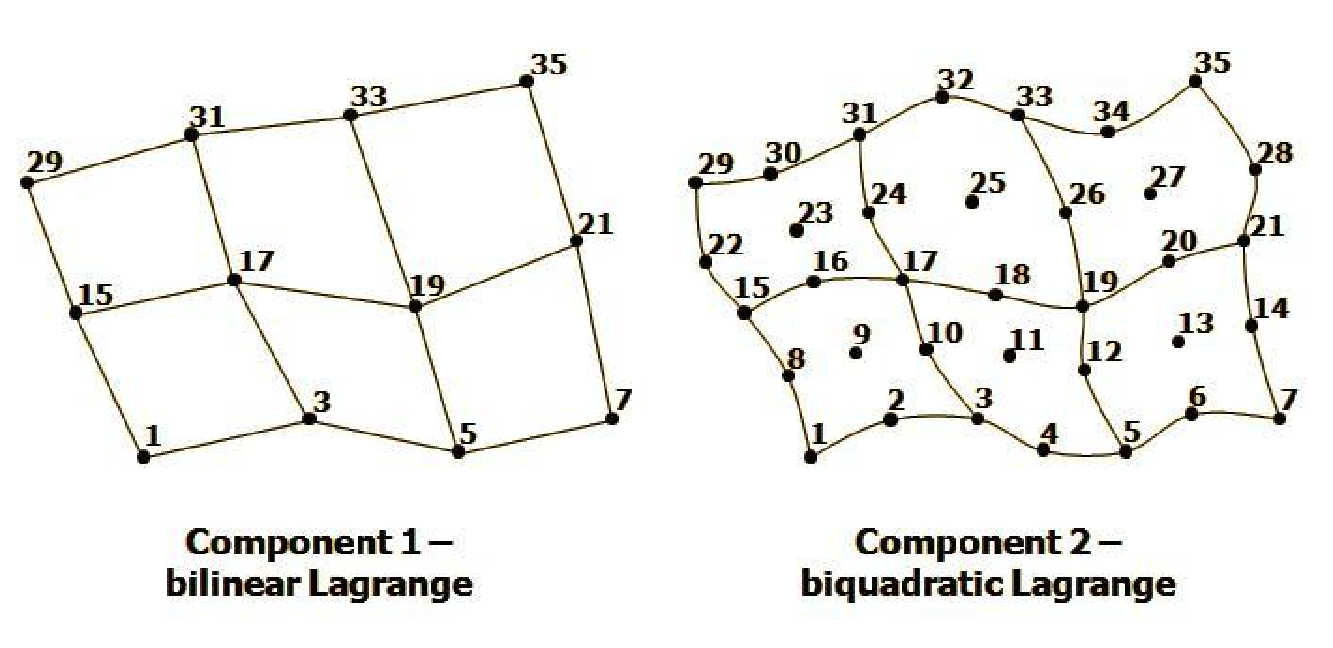
\includegraphics[width=1\textwidth]{figs/Modules/mesh_components.eps}
\caption{Diagram showing the multiple mesh components of a mesh.}
\label{mesh_components}
\end{figure}

The \emph{ParMETIS} library (\emph{ParMETIS} is a parallel graph partitioning 
library) is used to calculate the decomposition of the mesh by element into 
domains. The resulting local topology of the domain is calculated in this 
module for the elements, lines, faces and dofs.

Two further sets of properties calculated in these routines are the adjacent 
and surrounding topology. Surrounding elements, faces and lines are node 
properties, they are defined as what elements, faces and lines a node is part 
of. Adjacent elements, lines and faces are element properties, they are defined 
as what elements, faces and lines are connected to an element through node 
connectivity. Adjacent elements are used to calculate the boundary of the mesh.


\section{Module: \\ \emph{multi\_compartment\_transport\_routines}}
\label{sec:multicompartmenttransportroutines}

The routines in this module handle the multi compartment transport model for 
volume coupling. The physical model describes the transport of a scalar 
concentration in, and between, multiple compartments, using the diffusion 
and advection-diffusion equations. Only the setup related to the problem and 
solvers is implemented in this routine, the setup related to the equations 
is kept in the respective \emph{equations\_routines} module. 


\section{Module: \emph{multi\_physics\_routines}}
\label{sec:multiphysicsroutines}

The routines in this module are for dealing with coupled problems.


\section{Module: \emph{node\_routines}}
\label{sec:noderoutines}

Nodes in \emph{OpenCMISS} store the nodal information. Nodes are 
associated with either an interface or a region, and have both a global 
and a user number (allowing the user to define their own numbering scheme 
to the nodes). In \emph{OpenCMISS} nodes are just labels for dofs, they 
do not have a position. The position in space of a dof is a property of 
the field. Dofs are important in \emph{OpenCMISS}, they are the basic 
topological unit, they are the basic unit by which matrices are indexed 
and calculations performed.


\section{Module: \emph{opencmiss}}
\label{sec:opencmiss}

The opencmiss module handles the bindings, the routines in this module act as 
an interface layer between the calls from the example program and the main 
\emph{OpenCMISS} library routines. The use of this layer allows the further 
extension of the code to enable other languages to call the main library 
routines (for example: \emph{C} and \emph{Python}).


\section{Module: \emph{problem\_constants}}
\label{sec:problemconstants}

This module is used to store the constants used by routines in the 
\emph{problem\_routines} module they are separated out from other 
constants to avoid circular model dependency.


\section{Module: \emph{problem\_routines}}
\label{sec:problemroutines}

Problems are separated from the equations. The problem routines are the 
numerical workflow to solve the physics of the problem. A problem has control 
loops, control loops are described further in the description of the 
\emph{control\_loop\_routines}.

Nested control loops allow the dealing of problem complexity, each control 
loop can have a number of different solvers.

Coupled problems can be multiple problems in the same region or multiple 
regions together solving one problem.


\section{Module: \emph{region\_routines}}
\label{sec:regionroutines}

Regions are one of the primary objects in \emph{OpenCMISS}, they encapsulate 
the modelling object and are a construct allowing the modelling of multiple 
areas, either of different biological organs or of separate physics. They act 
as a base container and namespace for fields, equations etc. Fields need to 
have unique user numbers within a region, across different regions however 
this distinction is unnecessary. Regions can be labelled with a unique user 
defined number. 

Regions are hierarchical in nature, a region can have one parent region and a 
number of daughter sub-regions. Daughter regions are related in space to 
parent regions by an origin and an orientation of the regions coordinate 
system. Daughter regions may only have the same or fewer dimensions as the 
parent region. All regions are defined with respect to a parent region, the 
exception is the global (world) region (number $0$) which is defined with a 
parent region of itself' and has the global (world) coordinate system.
  
The fields, meshes, data points, coordinate system, nodes, sub-regions and 
interfaces are directly attached to the region object. When a region is 
initialised the objects contained in the region such as the meshes, generated 
meshes, equations sets and interfaces are also initialised. Together with the 
start, initialise, destroy and finalise routines, the region routines allow 
the setting to a region of multiple regions, each indexed by region user 
numbers.


\section{Module: \emph{solver\_mapping\_routines}}
\label{sec:solvermappingroutines}

\emph{OpenCMISS} can solve linear or nonlinear problems. If the problem has 
both nonlinear and linear parts, \emph{OpenCMISS} solves the linear parts 
of the problem as a subset of the nonlinear part.

The data that has been assembled in the equations matrix needs to be assembled 
into the solver matrix. The routines in this module handle the mapping and 
assembly of the equation rows to the solver matrix $A$ (the amplification 
matrix), and the assembly of the $x$ vector, $b$ vector and the \emph{Jacobian} 
(for a nonlinear problem). The solver matrix $A$ is constructed from a 
combination of the mass matrix $M$, the damping matrix $C$ and the stiffness 
matrix $K$. An equation row can be mapped to one or more solver rows and 
vice-versa. The default is one-to-one mapping, mapping of many-to-one or 
one-to-many solver rows is used in strong coupling between differing physics.

The construction of the solver matrix can either be monolithic, in the case of
volume coupling where two (or more physics) are to be solved over a space, or
constructed from a combination of one or more separate matrices (in the case of
surface coupling and some physics types). The surface coupling method (that
uses the interface object) uses the Lagrange multiplier interface method as 
default.

For time dependent problems (all fluid problems) each time step is integrated 
over the time interval, with the corresponding weighting (shown by $\alpha$, 
$\beta$ and $\gamma$): $A=\alpha M + \beta C+ \gamma K$ \\
For non-time dependent problems there is no mass matrix.

When solving in a time loop the previous values are updated using the current
values at the end of the time loop, this is done at the end of post-solve
control loop.

Parallelisation of the solver matrix across processors is made by splitting up
the solver matrix $A$ by rows and columns. For the splitting of the matrix by
rows the same splitting scheme used to divide the equation matrix rows between
processors is used to divide up the solver matrix between processors. A global
numbering scheme is given in solver routines for the solver matrix rows.

In solver routines the ghost rows in the equation matrix rows are dropped, 
whilst the ghost columns persist and carry through to the solver matrix rows.

The main routine in this module is the \emph{solver mapping calculate} routine,
this routine calculates the solver mappings. This routine performs the 
following steps:

\begin{enumerate}
 \item Calculate the interface conditions that influence the equations set.
 \item Determine the number of rows in the solver matrix by creating lists of 
rows for each rank, allowing the rows to be arranged in rank order. The number 
of local and global rows in the solver matrix are calculated. If all the dofs 
in a row are set to fixed boundary condition then the row is not included in 
the solver matrix. Note: couplings are not defined at the moment there is only 
a 1-1 mapping, and similarly only 1-1 mapping between rows and dofs is 
available. 
 \item Loop over the rows in rank order and calculate the equations matrix row
to solver matrix row mappings for each row in rank order. There are no ghosted 
rows for the solver matrix so there is only one domain for the global to local 
map. 
 \item Calculate the number of local and global columns in the solver matrix by 
creating lists of columns for each rank, allowing the columns to be arranged in 
rank order. Allowing each solver column to be allocated to the equations sets 
mapping array and the solver mappings for each column to be calculated in rank 
order.
 \item Set up the column mappings such that the solver matrix (\emph{sm}) and 
equations matrix (\emph{em}) orderings are the same.
\end{enumerate}


\section{Module: \emph{solver\_matrices\_routines}}
\label{sec:solvermatricesroutines}

These routines handle the solver matrices which are the actually matrices to 
be solved for the numerical problem. Solver matrices are used with the solvers, 
either internal (the \emph{CMISS} solver) or external (\emph{PETSc}, 
\emph{GMRES}) solvers. \emph{OpenCMISS} has been setup to take full advantage of 
the optimised parallel features of the \emph{PETSc} numerical solver library, to  
allow the efficient operation of \emph{OpenCMISS} library in parallel.


\section{Module: \emph{solver\_routines}}
\label{sec:solverroutines}

Currently only finite element methods have been implemented in \emph{OpenCMISS}. 
Places holders have been made for other solution methods in \emph{OpenCMISS}.


\section{Module: \emph{sorting}}
\label{sec:sorting}

This module contains the routines used for sorting. A number sorting methods 
are available in \emph{OpenCMISS}: bubble, heap and shell sort. The default 
sorting method is heap sort. The sort methods sorts lists into ascending order. 


\section{Module: \emph{strings}}
\label{sec:strings}

This module contains the routines used for manipulating strings in 
\emph{OpenCMISS}.


\section{Module: \emph{trees}}
\label{sec:trees}

Binary search trees are used in \emph{OpenCMISS} to match a user-defined node 
number to a global or a local number of a node. \emph{Red-black} binary trees 
are used, as they have good order properties for lookups, searching and 
ordering, and good worst case characteristics. Trees are composed of keys and 
data, the search is made on the key and the return is whatever is required.

Nodes have a user node number assigned by the user and a corresponding 
global/local number that the program uses. User node numbers are used in the 
example file to reference the nodes in the mesh, their use allows users 
flexibility in their ordering and referencing of the nodes. Presently trees 
are only used for nodes lookup.

Trees are used in \emph{OpenCMISS} by two objects: the \emph{mesh object} uses 
trees to lookup the global node number, whilst the \emph{domain object} uses
trees to lookup the local node number.


\section{Module: \emph{types}}
\label{sec:types}

The \emph{types} module holds the all data types definitions and type
relationships used in the \emph{OpenCMISS} library. Comments are provided 
in this module on each of the types defined. The types are located in this 
module in order to avoid cyclic dependency. 
